%-------------------------------------------------------------------------------------------------------
%-------------------------------------------------------------------------------------------------------
% Sec & Label

\section{Introduction}
\label{sec:introduction}

%-------------------------------------------------------------------------------------------------------
%-------------------------------------------------------------------------------------------------------


The objective of this laboratory assignment is to optimize and study an AC/DC converter
circuit. We were given total freedom to choose the architecture of the Envelope Detector
and Voltage Regulator circuits. Our goal is to achieve the highest merit($M$) possibe. This
value is obtained with the following equations:
	
\[
M = \frac{1}{cost\times (Ripple(vout) + avg(vout-12) + 10^{-6})}
\]

\[
 cost = cost_{resistors} + cost_{capacitor} + cost_{diodes} 
\]

$cost_{resistors} = 1MU/kOhm$; $cost_{capacitors} = 1MU/\mu- F$;
$cost_{diodes} = 0.1MU/diode$ \\

For reasons explained later, our circuit (in total) contains:

\begin{itemize}
	\item one voltage source ($V_1$)
	\item two inductors ($L_1$,$L_2$)
	\item one resistor ($R_1$)
	\item one capacitor ($C_1$)
	\item twenty diodes ($D_1$-$D_{20}$)
\end{itemize}

In Section \ref{sec:analysis}, a theoretical analysis of the circuit is presented. In
Section \ref{sec:simulation} , the circuit is analysed by simulation, and the results are
compared to the theoretical results obtained in Section \ref{sec:analysis}. The conclusions
of this study are outlined in Section \ref{sec:conclusion}.


\begin{figure}[h]
	\centering
	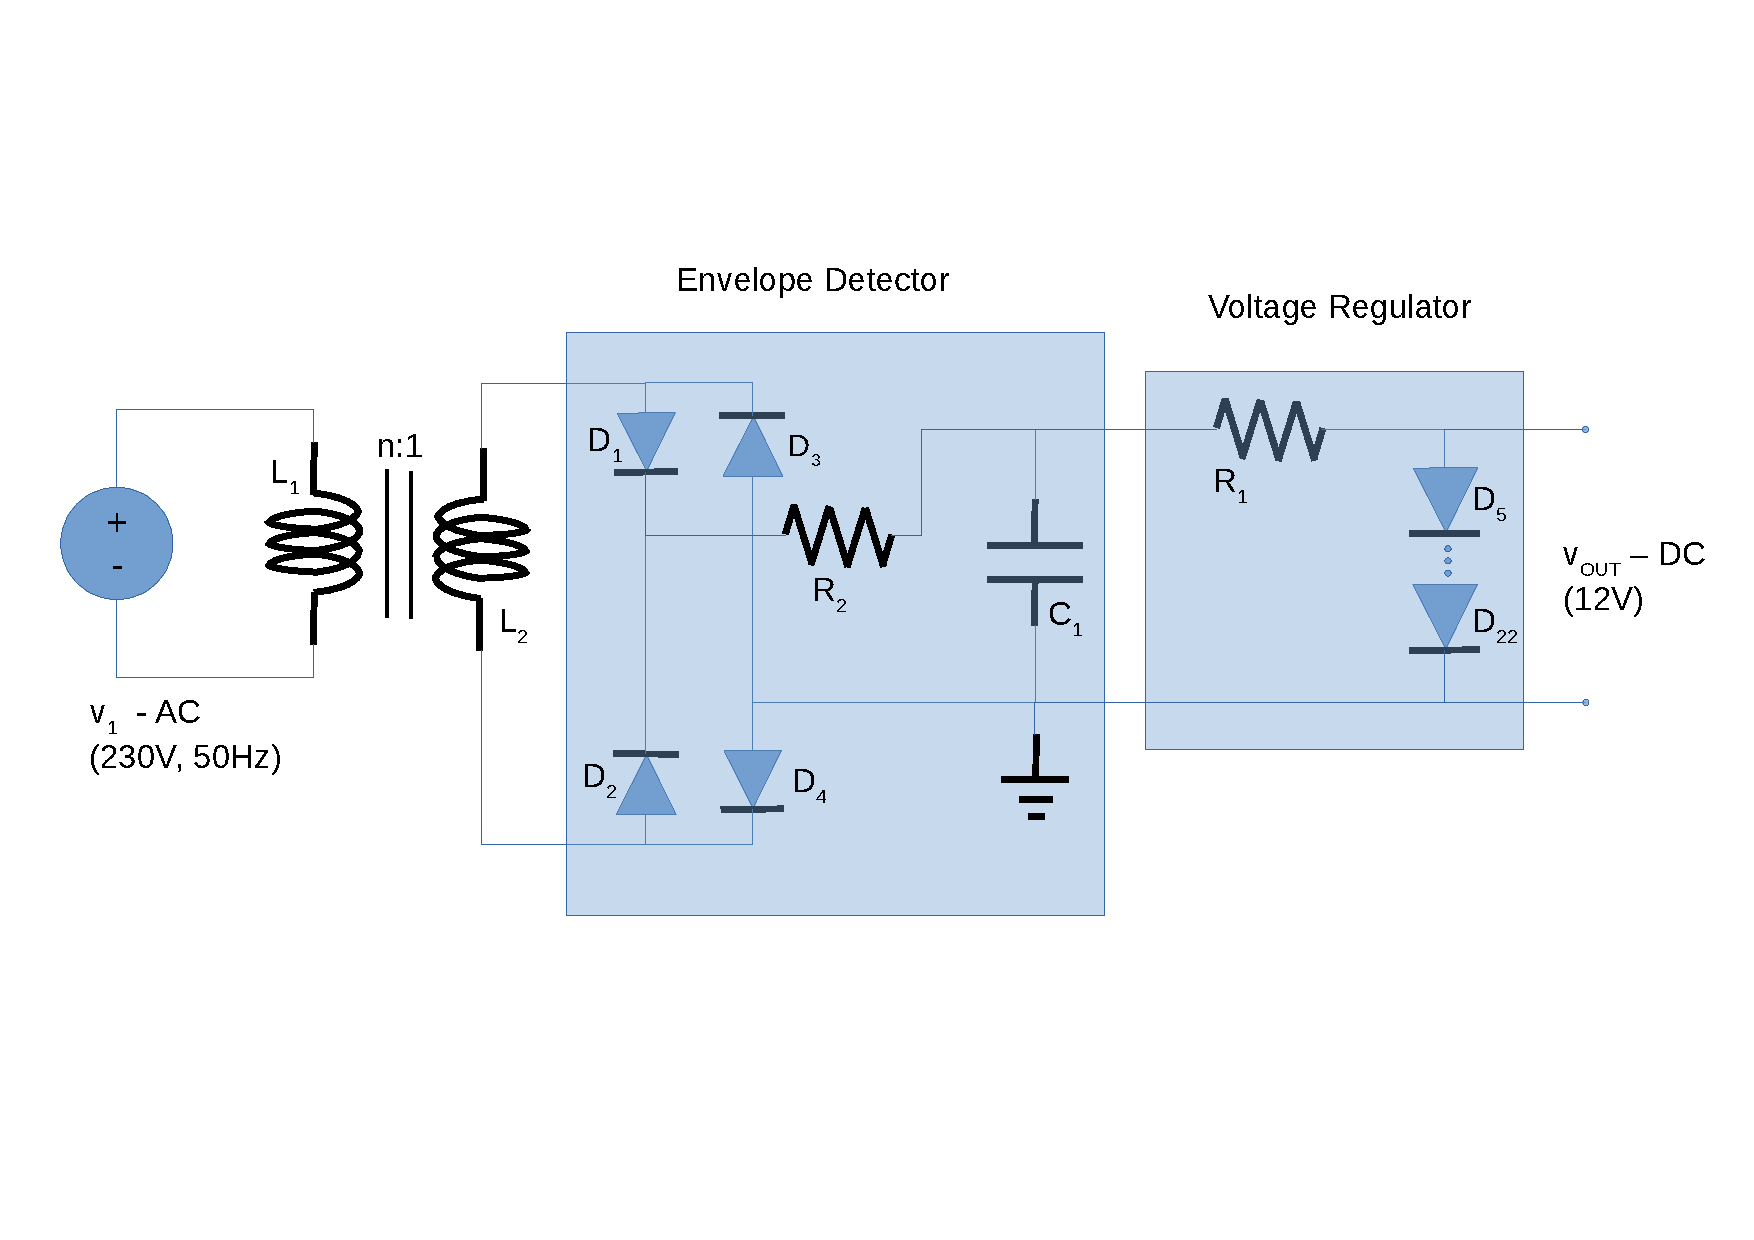
\includegraphics[width=0.85\linewidth]{dsnh_t3.pdf}
	\caption{Circuit T3}
\label{fig:Desenho_t3}
\end{figure}


